
% !TEX root = journal_02.tex
\documentclass[12pt,a4paper]{article}

% ---------------------------------------------------------
% Packages
% ---------------------------------------------------------

\usepackage[a4paper,margin=1in]{geometry}
\usepackage[T1]{fontenc}
\usepackage{newtxtext,newtxmath}
\usepackage{setspace}
\usepackage{enumitem}
\usepackage{booktabs}
\usepackage{array}
\usepackage{longtable}
\usepackage{graphicx}
\usepackage{float}
\usepackage{titlesec}
\usepackage{fancyhdr}
\usepackage[hidelinks]{hyperref}

% ---------------------------------------------------------
% Document formatting
% ---------------------------------------------------------

\setstretch{1.12}

\setlength{\parindent}{0pt}
\setlength{\parskip}{6pt}

\titleformat{\section}
{\large\bfseries}
{\thesection.}{0.5em}{}

\titleformat{\subsection}
{\normalsize\bfseries}
{\thesubsection}{0.5em}{}

\pagestyle{fancy}
\fancyhf{}
\fancyfoot[C]{\thepage}
\renewcommand{\headrulewidth}{0pt}

% ---------------------------------------------------------
% Document
% ---------------------------------------------------------

\begin{document}

% ---------------------------------------------------------
% Title Page
% ---------------------------------------------------------

\begin{titlepage}

\centering

\vspace*{0.8in}

{\Large\bfseries Smart City Civic Complaint and Management System\par}

\vspace{0.25in}

{\large\bfseries Software Engineering Project Journal -- 02\par}

\vspace{0.8in}

\textbf{Submitted to:}\par

Nisha Thakur\par

Thapar Institute of Engineering and Technology\par

\vspace{0.45in}

\textbf{Submitted by:}\par

Hittin Gupta [1024170437]\par

\vfill

\textbf{Journal 02}\par

Requirements Analysis and System Modelling\par

September 2026

\end{titlepage}

% ---------------------------------------------------------
% 1. Objective
% ---------------------------------------------------------

\section{Objective}

The objective of this journal is to document the requirements analysis and system modelling activities carried out for the Smart City Civic Complaint and Management System.

The main objectives were:

\begin{itemize}[leftmargin=*]

\item To understand the functional requirements of the proposed civic complaint management system.

\item To identify the major actors involved in the system and understand their responsibilities.

\item To analyze the major use cases associated with citizens, department officers, field workers, and administrators.

\item To understand the complete lifecycle of a civic complaint from submission to resolution and closure.

\item To study the Use Case Diagram and Activity Diagram prepared for the project.

\item To review the project Gantt Chart and understand the planned development schedule.

\item To organize and understand the existing project artifacts before proceeding with implementation.

\end{itemize}

% ---------------------------------------------------------
% 2. Work Completed
% ---------------------------------------------------------

\section{Work Completed}

Following the completion of the project proposal, the next stage involved understanding the functional requirements and modelling the proposed system.

The project requirements and existing Software Engineering artifacts were studied to obtain a clearer understanding of the system before implementation.

The major activities covered in this journal were:

\begin{enumerate}[leftmargin=*]

\item Requirements analysis

\item Identification of system actors

\item Identification of functional requirements

\item Analysis of major use cases

\item Study of the complaint management workflow

\item Review of the Use Case Diagram

\item Review of the Activity Diagram

\item Review of the project Gantt Chart

\item Organization of project artifacts in the GitHub repository

\end{enumerate}

These activities provide a foundation for the implementation and testing stages of the project.

% ---------------------------------------------------------
% 3. System Overview
% ---------------------------------------------------------

\section{System Overview}

The Smart City Civic Complaint and Management System is a web-based platform designed to provide a structured mechanism for citizens to report civic issues and track their resolution.

The system connects citizens with department officers and field workers through a centralized complaint management workflow.

A complaint can contain information such as:

\begin{itemize}[leftmargin=*]

\item Complaint category

\item Description of the problem

\item Location

\item Photograph or other supporting evidence

\end{itemize}

After submission, the complaint is reviewed by a department officer. Once verified, it can be assigned to a field worker for resolution. The field worker performs the required work, updates progress, and uploads evidence of the completed work.

The citizen can subsequently verify the resolution and provide feedback. If the issue has not been properly resolved, the complaint can be reopened.

This creates a traceable workflow from complaint creation to final resolution.

% ---------------------------------------------------------
% 4. System Actors
% ---------------------------------------------------------

\section{System Actors}

The system consists of four major user roles.

\begin{longtable}{p{0.25\textwidth} p{0.65\textwidth}}

\toprule

\textbf{Actor} & \textbf{Main Responsibilities} \\

\midrule

Citizen &
Register or log in, submit complaints, provide complaint details and location, upload photographs, track complaint status, verify resolution, provide feedback, and reopen complaints when required. \\

Department Officer &
Review submitted complaints, verify complaints, assign field workers, monitor progress, and manage complaint status. \\

Field Worker &
View assigned tasks, accept work, travel to the complaint location, perform the required work, update progress, upload before/after evidence, and mark the work as completed. \\

Administrator &
Manage users, departments, and workers, monitor complaints, monitor SLA-related information, and view system-level analytics. \\

\bottomrule

\end{longtable}

The identification of these actors helps define the responsibilities and access requirements of different users within the system.

% ---------------------------------------------------------
% 5. Functional Requirements
% ---------------------------------------------------------

\section{Functional Requirements}

The major functional requirements identified for the system are divided according to the responsibilities of each user role.

\subsection{Citizen Requirements}

The citizen should be able to:

\begin{itemize}[leftmargin=*]

\item Register and log in to the system.

\item Submit a new civic complaint.

\item Select an appropriate complaint category.

\item Enter a description of the issue.

\item Provide the location of the complaint.

\item Upload a photograph as supporting evidence.

\item Receive a unique complaint ID.

\item Track the status of a submitted complaint.

\item Verify whether the reported issue has been resolved.

\item Provide feedback or rating after resolution.

\item Reopen a complaint when the issue has not been resolved satisfactorily.

\end{itemize}

\subsection{Department Officer Requirements}

The department officer should be able to:

\begin{itemize}[leftmargin=*]

\item View newly submitted complaints.

\item Review complaint details, photographs, and location.

\item Verify whether a complaint is valid.

\item Reject invalid complaints with an appropriate reason.

\item Assign verified complaints to field workers.

\item Monitor work progress.

\item Update complaint status when required.

\end{itemize}

\subsection{Field Worker Requirements}

The field worker should be able to:

\begin{itemize}[leftmargin=*]

\item View assigned tasks.

\item Accept an assigned task.

\item View the complaint location and details.

\item Update work progress.

\item Upload before and after photographs as evidence.

\item Mark the assigned work as completed.

\end{itemize}

\subsection{Administrator Requirements}

The administrator should be able to:

\begin{itemize}[leftmargin=*]

\item Manage system users.

\item Manage departments.

\item Manage field workers.

\item Monitor complaints.

\item Monitor service-level information.

\item View analytics related to complaints and system activity.

\end{itemize}

% ---------------------------------------------------------
% 6. Use Case Analysis
% ---------------------------------------------------------

\section{Use Case Analysis}

The Use Case Diagram was analyzed to understand the interaction between the system and its external actors.

The major use cases identified for the system include:

\begin{itemize}[leftmargin=*]

\item Register / Login

\item Submit Complaint

\item Track Complaint Status

\item Verify Resolution

\item Provide Feedback

\item Reopen Complaint

\item Select Category

\item Enter Description

\item Provide Location

\item Generate Complaint ID

\item Upload Photograph

\item Review Complaint

\item Verify Complaint

\item Assign Worker

\item Monitor Progress

\item Manage Complaint Status

\item View Assigned Tasks

\item Accept Work

\item Update Work Progress

\item Upload Evidence

\item Mark Work Completed

\item Manage Users

\item Manage Departments

\item Manage Workers

\item Monitor Complaints

\end{itemize}

The Use Case Diagram also includes the planned Smart Assistance layer. This layer contains:

\begin{itemize}[leftmargin=*]

\item Smart Classification

\item Duplicate Detection

\item Priority Calculation

\end{itemize}

These smart features are intended to improve the efficiency of complaint processing after the core complaint workflow has been established.

% ---------------------------------------------------------
% 7. Use Case Diagram
% ---------------------------------------------------------

\section{Use Case Diagram}

The Use Case Diagram provides a functional view of the proposed system by showing the major actors and their interactions with the system.

The diagram distinguishes the responsibilities of citizens, department officers, field workers, and administrators.

\begin{figure}[H]
\centering
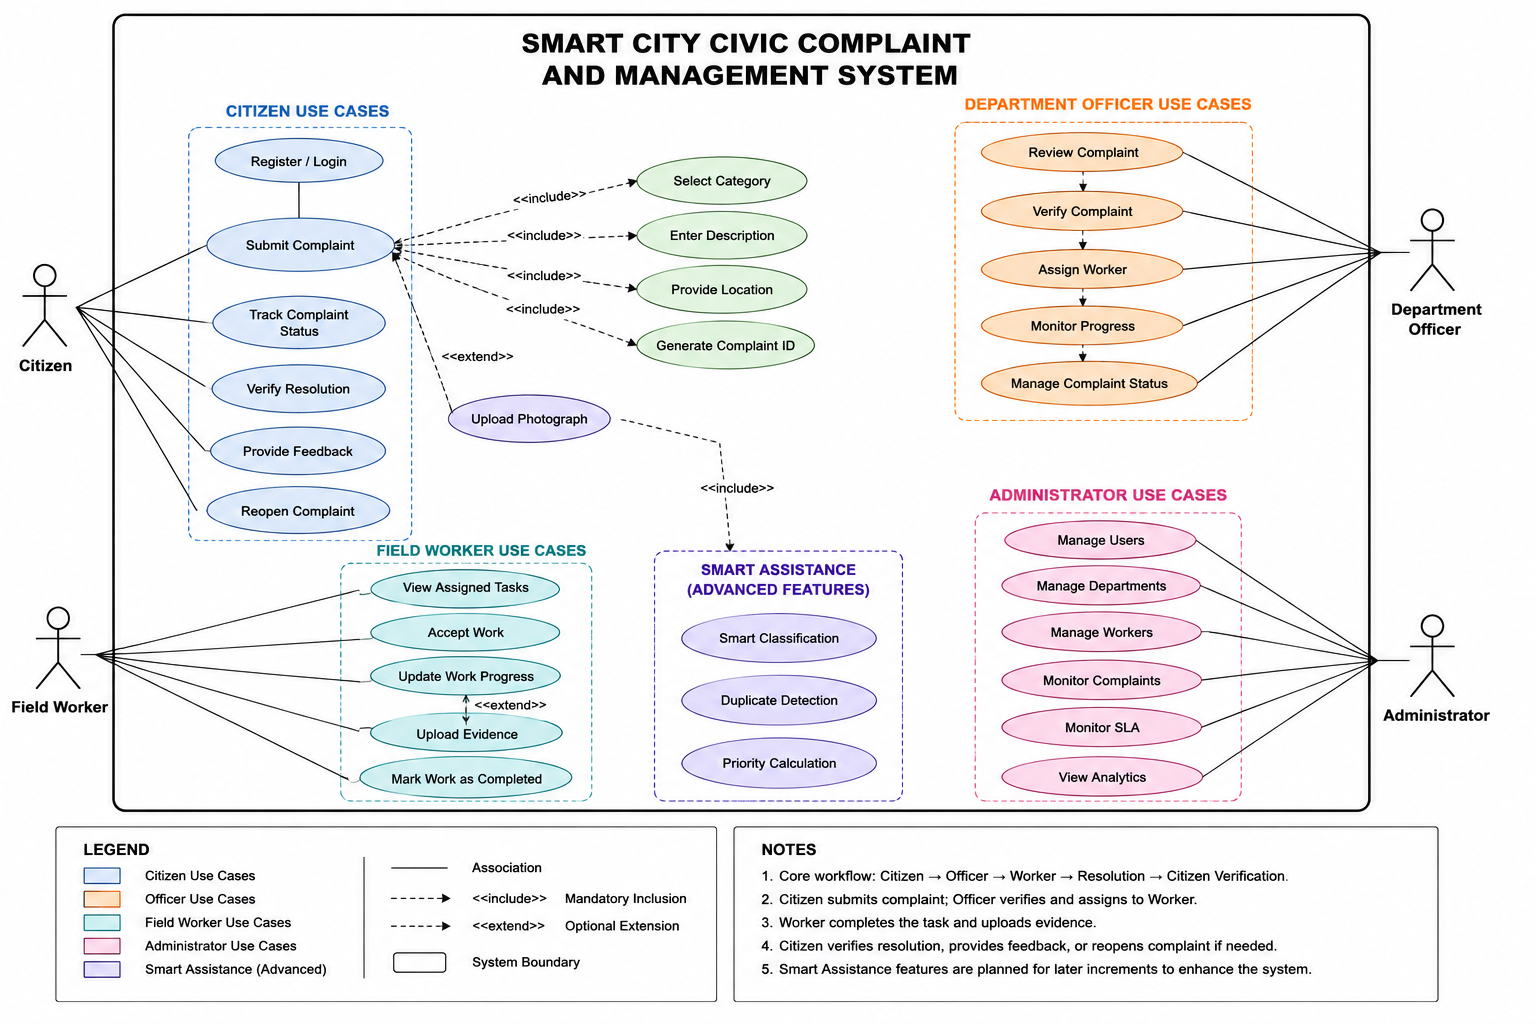
\includegraphics[width=\textwidth]{../../assets/use-case.png}
\caption{Use Case Diagram of the Smart City Civic Complaint and Management System}
\label{fig:usecase}
\end{figure}

The diagram helps establish the system boundary and provides a reference for the functionality that will be implemented during development.

% ---------------------------------------------------------
% 8. Activity Diagram
% ---------------------------------------------------------

\section{Activity Diagram Analysis}

The Activity Diagram was studied to understand the sequence of activities involved in processing a complaint.

The major stages of the workflow are:

\begin{enumerate}[leftmargin=*]

\item Citizen registration or login.

\item Submission of a civic complaint.

\item Validation of the submitted information.

\item Generation of a complaint ID.

\item Storage of the complaint in the database.

\item Setting the complaint status to ``Submitted''.

\item Notification of the department officer.

\item Review and verification of the complaint.

\item Assignment of a field worker.

\item Field worker acceptance of the task.

\item Execution of the required work.

\item Updating of work progress.

\item Uploading of before and after evidence.

\item Marking the work as completed.

\item Updating the complaint status.

\item Notification of the citizen.

\item Citizen verification of the resolution.

\item Closure of the complaint if the issue is resolved.

\item Reopening of the complaint if the issue remains unresolved.

\end{enumerate}

\begin{figure}[H]
\centering
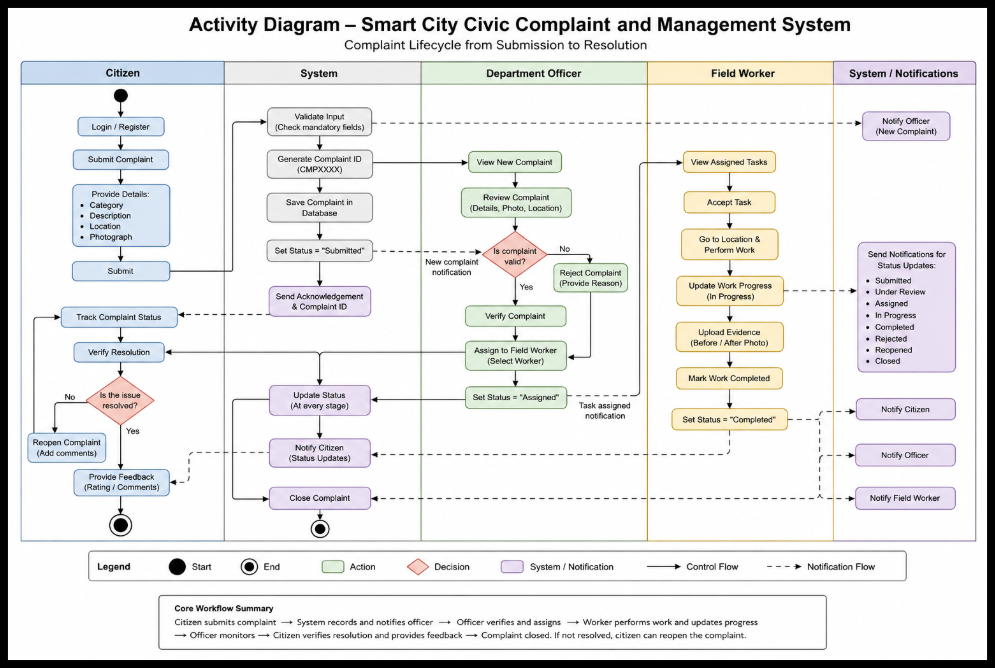
\includegraphics[width=\textwidth]{../../assets/activity-diagram.png}
\caption{Activity Diagram of the Complaint Lifecycle}
\label{fig:activity}
\end{figure}

The activity diagram provides a process-oriented view of the system and complements the functional information represented in the Use Case Diagram.

% ---------------------------------------------------------
% 9. Core Workflow
% ---------------------------------------------------------

\section{Core Complaint Workflow}

The complete complaint lifecycle identified during the analysis can be represented as:

\[
\text{Citizen}
\rightarrow
\text{Complaint Submission}
\rightarrow
\text{Officer Verification}
\rightarrow
\text{Worker Assignment}
\rightarrow
\text{Work and Evidence}
\rightarrow
\text{Resolution}
\rightarrow
\text{Citizen Verification}
\]

The workflow provides traceability throughout the complaint lifecycle.

If the complaint is valid, the department officer verifies it and assigns it to an appropriate field worker.

The field worker then performs the required work and uploads evidence. After the work is completed, the citizen is notified and can verify the resolution.

If the citizen is not satisfied with the resolution, the complaint can be reopened for further action.

% ---------------------------------------------------------
% 10. Project Schedule
% ---------------------------------------------------------

\section{Project Schedule}

The project Gantt Chart was reviewed to understand the planned development schedule.

The project follows an incremental development approach in which the core complaint workflow is prioritized before implementing advanced smart features.

The major planned milestones include:

\begin{itemize}[leftmargin=*]

\item W4 -- Project Proposal and Report Submission

\item W7 -- Prototype and Report Submission

\item W8 -- Improvement Plan

\item W9--W10 -- MST Week

\item W11--W12 -- Progress Monitoring

\item W13 -- Buffer

\item W14 -- Progress Monitoring

\item W15 -- Diwali Break

\item W16 -- Progress Monitoring over the second prototype

\item W17 -- Final Prototype, Presentation and Report Submission

\item W18 -- Assessment Week / Buffer

\item W19--W20 -- EST Week

\end{itemize}

\begin{figure}[H]
\centering
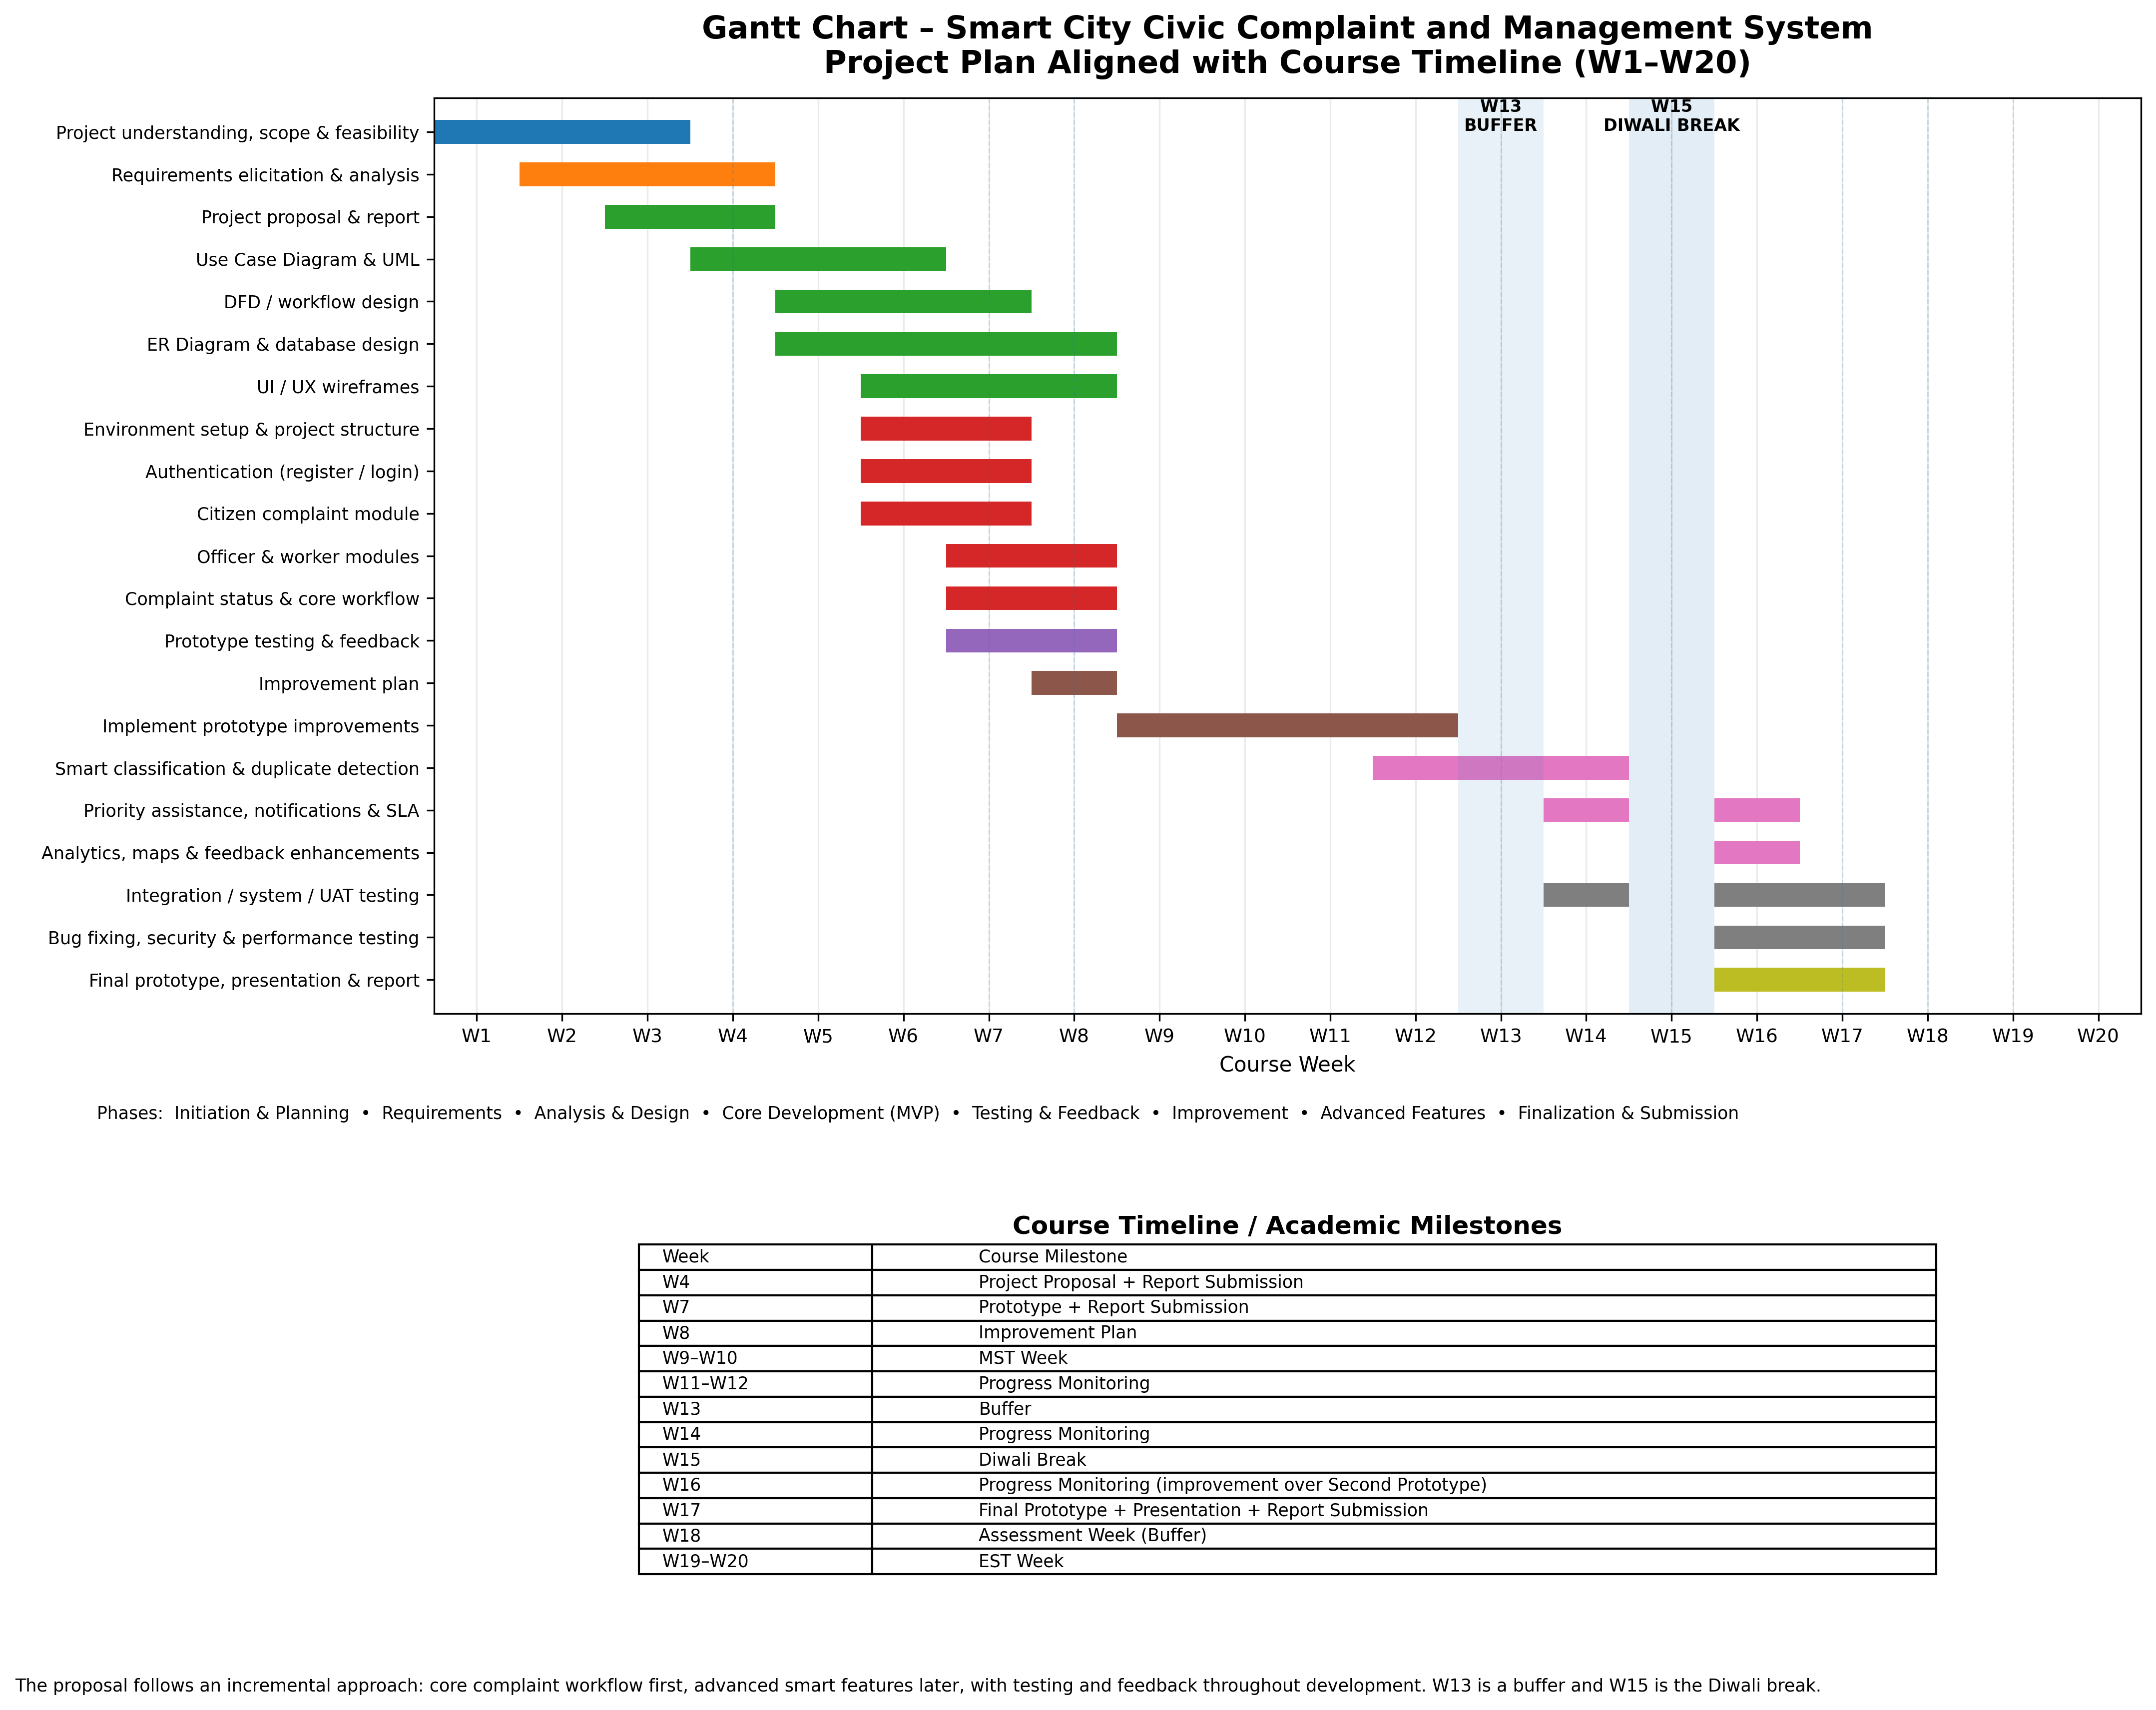
\includegraphics[width=\textwidth]{../../assets/gantt-chart.png}
\caption{Project Gantt Chart}
\label{fig:gantt}
\end{figure}

The schedule provides a reference for organizing implementation, testing, improvement, and final submission activities.

% ---------------------------------------------------------
% 11. Repository Organization
% ---------------------------------------------------------

\section{Repository Organization}

The project artifacts are organized in the GitHub repository using separate folders for source material, documentation, and project journals.

The current organization includes:

\begin{verbatim}
SOFTWARE-ENGINEERING/

    assets/
        activity-diagram.png
        gantt-chart.png
        use-case.png

    docs/
        activity-diagram.pdf
        gantt-chart.pdf
        use-case.pdf

    frontend/

    journals/
        1024170429_achintya/
        1024170437_hittin/

    project_proposal/

    README.md
\end{verbatim}

The \texttt{assets} directory contains visual project artifacts, while the \texttt{docs} directory contains printable documentation versions.

The \texttt{journals} directory maintains individual project journals for the team members.

The repository is maintained using Git and GitHub to support collaborative development and version control.

% ---------------------------------------------------------
% 12. Software Engineering Understanding
% ---------------------------------------------------------

\section{Software Engineering Understanding}

The requirements analysis and system modelling activities provided an understanding of how a software system can be divided into actors, functional requirements, and workflows before implementation.

The Use Case Diagram provides an understanding of \emph{who interacts with the system and what functions they perform}.

The Activity Diagram provides an understanding of \emph{how a complaint moves through the system from submission to closure}.

The Gantt Chart provides an understanding of \emph{when different development activities are planned}.

Together, these artifacts provide complementary views of the same software project.

The analysis also highlighted the importance of defining responsibilities for different user roles before implementing authentication, authorization, database operations, and user interfaces.

% ---------------------------------------------------------
% 13. Result
% ---------------------------------------------------------

\section{Result}

The following activities were completed as part of the requirements analysis and system modelling stage:

\begin{table}[H]

\centering

\begin{tabular}{p{0.62\textwidth} p{0.20\textwidth}}

\toprule

\textbf{Activity} & \textbf{Status} \\

\midrule

System requirements analyzed & Completed \\

Major system actors identified & Completed \\

Functional requirements identified & Completed \\

Major use cases analyzed & Completed \\

Complaint workflow understood & Completed \\

Use Case Diagram reviewed & Completed \\

Activity Diagram reviewed & Completed \\

Project Gantt Chart reviewed & Completed \\

Repository organization reviewed & Completed \\

\bottomrule

\end{tabular}

\end{table}

% ---------------------------------------------------------
% 14. Learning
% ---------------------------------------------------------

\section{Learning / Engineering Understanding}

This activity helped develop an understanding of the relationship between requirements, system modelling, and implementation.

It was observed that a clear definition of system actors and functional requirements is important before starting implementation.

The analysis of the complaint lifecycle also helped in understanding how different modules of the application will interact.

For example, complaint submission will eventually interact with authentication, database storage, location and image handling, complaint tracking, officer verification, worker assignment, notifications, and resolution verification.

The modelling activities therefore provide a foundation for the development of the frontend, backend, database, and future smart assistance modules.

% ---------------------------------------------------------
% 15. Conclusion
% ---------------------------------------------------------

\section{Conclusion}

Journal 02 documents the requirements analysis and system modelling activities for the Smart City Civic Complaint and Management System.

The major system actors, functional requirements, use cases, and complaint lifecycle were identified and analyzed.

The Use Case Diagram, Activity Diagram, and Gantt Chart provided different perspectives of the project by representing system functionality, process flow, and development planning respectively.

The analysis establishes a clearer understanding of the system before implementation. The next stages of development can therefore build upon the defined requirements and workflow while maintaining consistency with the established project scope.

\end{document}